
\section{SU(2)$_L \otimes$U(1)$_V$ (Glashow, 1961)}
%
In the previous section we saw that in order to avoid unitarity violation we need to construct a gauge theory for the $W^\pm$ bosons. This must be:
\begin{itemize}
\item non-abelian, because abelian gauge bosons ($\gamma$) are neutral,
\item massive (how do we achieve this?).
\end{itemize}
The weak current $\frac{1}{2} J_\mu = \bar{\nu}_e\gamma_\mu e_L + ...$ is built out of left-handed doublets:

\[ \psi_L \equiv \left( \begin{array}{cc}
\nu_e   \\
e   \end{array} \right)_L, \qquad
  \\ \left( \begin{array}{cc}
 \nu_\mu \\
\mu   \end{array} \right)_L, \qquad  \\ 
\left( \begin{array}{cc}
 \nu_\tau \\
\tau   \end{array} \right)_L \qquad\] 
and right-handed singlets 
$\psi_R \equiv e_R, \mu_R, \tau_R$. Notice that there is no $\nu_R$ because $\nu$ are massless. For now we are ignoring the quarks, and focussing on formulating a "theory of leptons". One obvious gauge group is SU(2) (or \textit{weak isospin}), with the $\psi_L$ and the $\psi_R$ in different representations because the weak interaction is \textit{chiral}. More explicitly,
\begin{equation}
\psi_L \to U \psi_L \qquad \text{and} \qquad \psi_R \to \psi_R, \qquad \text{where} \qquad U=\exp\bigg(\frac{i}{2}\underline{\alpha}\cdot\underline{\tau}\bigg) \in \text{SU(2)}.
\end{equation}
The dimension of SU(2) is 3, so there will be three gauge bosons. The hope is that these will correspond to $W^\pm, \gamma$. 

To see how the theory works in practice, consider explicitly writing

\[ \bar{\nu}_e\gamma_\mu e_L= \left( \begin{array}{c}
\nu_e \ e_L   \end{array} \right)
  \\ \left( \begin{array}{cc}
 0 \ 1 \\
1 \ 0   \end{array} \right)\gamma_\mu \\ 
\left( \begin{array}{cc}
 \nu_e \\
e_L   \end{array} \right). \qquad\] 
Now note that 
\[ \left( \begin{array}{cc}
 0 \ 1 \\
0 \ 0   \end{array} \right) = \frac{1}{2} 
\left( \begin{array}{cc}
 0 \ 1 \\
1 \ 0   \end{array} \right) + \frac{i}{2}
\left( \begin{array}{cc}
 0 \ -i \\
i \ \ 0   \end{array} \right) = \frac{1}{2}(\tau_1 + i\tau_2) \equiv T^+.
\qquad\] 
So
\begin{equation}
\begin{split}
\frac{1}{2}J_\mu &= \bar{\psi}_L T^+ \gamma_\mu \psi_L \\
\text{and} \qquad \frac{1}{2}J_\mu^\dagger &= \bar{\psi}_L T^- \gamma_\mu \psi_L,
\end{split}
\end{equation}
where 
\[ T^- = \frac{1}{2}(\tau_1 - i\tau_2) =
  \\ \left( \begin{array}{cc}
 0 \ 0 \\
1 \ 0   \end{array} \right). \qquad\]
Then, using the SU(2) relations
\begin{equation}
\begin{split}
&[T^+,T^-] = 2T_3, \\
&[T_3, T^\pm] = \pm T^\pm \\
\text{where} \qquad &T_3 = \frac{1}{2}\tau_3,
\end{split}
\end{equation}
we can compute the commutator
\begin{equation}
\begin{split}
[J_0^\dagger, J_0] &= \psi_L^\dagger[T^+,T^-]\psi_L \\
&=\psi_L^\dagger \ 2T^3 \psi_L \\
&= 2J_0^3.
\end{split}
\end{equation}
So we have three weak Noether currents:
\begin{equation}
\begin{split}
\underline{J}_\mu = (J_\mu^1, J_\mu^2, J_\mu^3) = \bar{\psi}_L \underline{T} \psi_L, \qquad \underline{T} = \frac{1}{2}\sigma, \\
\text{with} \qquad J_\mu^\pm = \frac{1}{2}(J_\mu^1 \pm iJ_\mu^2), \qquad J_\mu = J_\mu^+, \qquad J_mu^\dagger = J_\mu^-.
\end{split}
\end{equation}
Transforming in the adjoint representation of SU(2)$_L$ (i.e. the fundamental representation of SO(3)), we find
\begin{equation}
J_\mu^3 = \frac{1}{2}(\bar{\nu}_e \gamma_\mu \nu_e - \bar{e}_L \gamma_\mu e_L).
\end{equation}
This has $\Delta Q =0$ so it is a neutral current. However, it is \textit{not} the electromagnetic neutral current:
\begin{equation}
j_\mu = - \bar{e}\gamma_\mu e = - \bar{e}_L \gamma_\mu e_L - \bar{e}_R \gamma_\mu e_R,
\end{equation}
because this is vector-like and does not involve any neutrinos.
Considering the electric charge operator, $Q$:
\[ Q \psi_L = \left( \begin{array}{cc}
0 & 0  \\
0 & -1  \end{array} \right) \psi_L, \qquad
Q \psi_R = - \psi_R, \]
we can write $Q = T_3 + Y$, where $Y = (-1/2) \mathds{1}$ for left-handed leptons, and $Y = -1$ for right-handed leptons. Decomposed in the representation,
\[ Q \qquad = \qquad T_3 \qquad + \qquad Y: \]
\[\left( \begin{array}{cc}
0 & 0  \\
0 & -1  \end{array} \right)=
\left( \begin{array}{cc}
1/2 & 0  \\
0 & -1/2  \end{array} \right) +
\left( \begin{array}{cc}
-1/2 & 0  \\
0 & -1/2  \end{array} \right). \]
We call $Y$ the "weak hypercharge". It generates a U(1) symmetry of the form
\begin{equation}
\psi_L \to e^{-1/2 i \beta}\psi_L,  \qquad \psi_R \to e^{-i \beta}  \psi_R.
\end{equation}
Again, note the chiral structure.

Clearly the generators of SU(2)$_L$ and U(1)$_Y$ commute: the full symmetry group is SU(2)$_L \otimes$U(1)$_Y$, with elements $\exp{(i \underline{\alpha} \cdot \underline{T} + i \beta Y)}$. Overall, the Noether current is made up of a part belonging to SU(2)$_L$ and a part belonging to U(1)$_Y$, so we can write:
\begin{equation}
J_\mu^Y = j_\mu - J_\mu^3 = - \frac{1}{2}(\bar{\nu}_e \gamma_\mu \nu_e + \bar{e}_L \gamma_\mu e_L) - (\bar{e}_R \gamma_\mu e_R).
\end{equation}
From this starting point we want to build an SU(2)$_L \otimes$U(1)$_Y$ gauge theory. Considering the two individual groups,
\begin{equation}
\begin{split}
&\text{SU(2)}_L: \qquad \text{coupling \ } g, \qquad \text{gauge fields \ } \mathcal{W}_\mu \equiv \underline{W}_\mu \cdot \underline{T} \\
&\text{U(1)}_Y: \qquad \text{coupling \ } g^\prime, \qquad \text{gauge fields \ } B_\mu.
\end{split}
\end{equation}
The local symmetries are:
\begin{equation}
\begin{split}
&\mathcal{W}_\mu \to u \mathcal{W}_\mu u^\dagger + ig\ u \partial_\mu u^\dagger \\
&B_\mu \to B_\mu + i g^\prime \partial_\mu \beta,
\end{split}
\end{equation}
which translate to the covariant derivatives (using the hypercharge assignments):
\begin{equation}
\begin{split}
\mathcal{D}_\mu \psi_L &= (\partial_\mu - ig \mathcal{W}_\mu + i g^\prime \frac{1}{2} B_\mu) \psi_L, \\
\mathcal{D}_\mu \psi_R &= (\partial_\mu + i g^\prime B_\mu) \psi_R.
\end{split}
\end{equation}
Recalling that $\bar{\psi}\slashed{\partial}\psi = \psi_L \slashed{\partial} \psi_L + \psi_R \slashed{\partial} \psi_R$, we can write the Lagrangian explicitly as:
\begin{equation} 
\label{eqn:20a}
\begin{split}
\mathcal{L}_D &= \bar{\psi}_L i \mathcal{D} \psi_L +  \bar{\psi}_R i \mathcal{D} \psi_R \\
&= \bar{\psi} i \slashed{\partial} \psi + g \underline{W}^\mu \bar{\psi} \underline{T} \gamma_\mu \psi_L - g^\prime B^\mu \bigg( \frac{1}{2} \bar{\psi}_L \gamma_\mu \psi_L + \bar{\psi}_R \gamma_\mu \psi_R \bigg) \\
& = \bar{\psi} i \slashed{\partial} \psi + g \underline{W}^\mu \cdot \underline{J}_\mu + g^\prime B^\mu J_\mu^Y.
\end{split}
\end{equation}
Let's consider the charged current terms. We can write the complex field $W$ in terms of two real fields $W_1$ and $W_2$:
\begin{equation}
W^\mu = \frac{1}{\sqrt{2}} (W_1^\mu + i W_2^\mu), \qquad W^{\mu \dagger} = \frac{1}{\sqrt{2}} (W_1^\mu - i W_2^\mu).
\end{equation}
Now let's evaluate the terms in Eqn. \ref{eqn:20a} in turn, using $T^\pm = (T_1 \pm iT_2)$ and $W^\pm = 1/\sqrt{2}(W_1 \pm iW_2)$:
\begin{equation} \label{eqn:20b}
\begin{split}
\underline{T} \cdot \underline{W}^\mu &= \frac{1}{2} (T_1 + i T_2) (W_1^\mu + i W_2^\mu) + \frac{1}{2} (T_1 - i T_2)(W_1^\mu + i W_2^\mu) + T_3 W_3^\mu \\
&= \frac{1}{\sqrt{2}} (T^+ W^{\mu \dagger} + T^- W^\mu) + T_3 W_3^\mu,\\
g \underline{W}^\mu \cdot \underline{J}_\mu &= \frac{1}{2 \sqrt{2}} g(W^{\mu \dagger} J_\mu + J_\mu^\dagger W^\mu) + gJ_\mu^3 W_3^\mu.
\end{split}
\end{equation}
Looking at the last line of Eqn. \ref{eqn:20b}, the term in brackets is the charged current interaction, and the $gJ_\mu^3 W_3^\mu$ term is a new addition. 

Now let's consider the neutral current and electromagnetic terms. Clearly neither $W_\mu^3$ nor $B_\mu$ alone is the photon. Instead, the photon is produced through a mixture of the two. In general, we can write:
\[\left( \begin{array}{cc}
W^\mu_3 \\
B^\mu 
\end{array} \right) =
 \left( \begin{array}{cc}
\cos\theta_w & \sin\theta_w  \\
-\sin\theta_w & \cos\theta_w  \end{array} \right) 
\left( \begin{array}{cc}
Z^\mu \\
A^\mu 
\end{array} \right), \]
where $\theta_w$ is the weak mixing or "Weinberg" angle, to be determined. Substituting this explicitly into the expressions above leads to:
\begin{equation}
\begin{split}
gJ_\mu^3W_3^\mu + g^\prime(j_\mu - J_\mu^3)B^\mu &= \bigg((g\sin\theta_w - g^\prime \cos\theta_w)J_\mu^3 + g^\prime \cos\theta_wj_\mu\bigg)A^\mu \\
&+ \bigg((g\cos\theta_w + g^\prime \sin\theta_w)J_\mu^3 - g^\prime \sin\theta_w j_\mu\bigg)Z^\mu \\
&= ej_\mu A^\mu + \frac{g}{\cos\theta_w}\bigg(J_\mu^3 - \sin^2\theta_w j_\mu \bigg)Z^\mu,
\end{split}
\end{equation}
where we have inferred that $e = g^\prime \cos\theta_w = g \sin\theta_w$ is the electric charge. The first term is the QED part and the second term is the neutral current part. Note that $g, g^\prime$ are the same order as $e$: in fact, according to \textit{electroweak unification}, $1/e^2 = 1/g^2 + 1/g^{\prime 2}$, i.e. $e = g g^\prime/\sqrt{g^2 + g^{\prime 2}}$.

All in all the complete interaction is:
\begin{equation}
\begin{split}
ej_\mu A^\mu + &\frac{1}{2\sqrt{2}}g\big(W^{\mu \dagger}J_\mu + J_\mu^\dagger W^\mu \big) + \frac{g}{2 \cos\theta_w} J_\mu^{NC}Z^\mu, \\
\text{where } \qquad J_\mu^{NC} &= 2(J_\mu^3 - \sin^2\theta_w j_\mu) \\
&= 2\bigg( \frac{1}{2} (\bar{\nu}_L \gamma_\mu \nu_L - \bar{e}_L \gamma_\mu e_L) + \sin^2\theta_w \bar{e} \gamma_\mu e \bigg) \\
&= \bar{\nu}_L \gamma_\mu \nu_L + \bar{e} \gamma_\mu \big( (2\sin^2\theta_w - \frac{1}{2}) + \frac{1}{2} \gamma^5 \big) e \\
&\equiv \bar{\nu}_L \gamma_\mu \nu_L + \bar{e} \gamma_\mu \big(c_V + c_A \gamma^5 \big)e.
\end{split}
\end{equation}
So the neutral current is not pure V-A, but instead a mixture of left and right:
\begin{equation}
\begin{split}
&c_V- c_A\gamma^5 = c_L P_L + c_R P_R \\
\text{where} \qquad &c_L = c_V + c_A = 2 \sin^2\theta_w -1, \qquad c_R = c_V-c_A = 2 \sin^2\theta_w.
\end{split}
\end{equation}
The Feynman rule corresponding to the neutral current vertex is
%
\newline
%\begin{wrapfigure}{l}{\linewidth}
  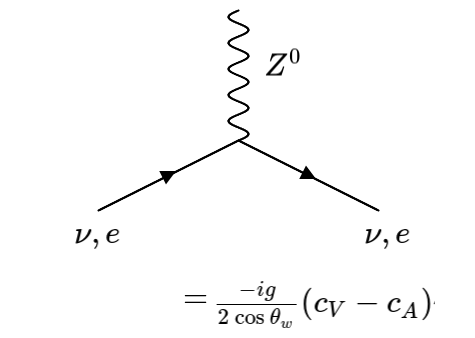
\includegraphics[width=0.4\linewidth]{figs/21a.png}
%\end{wrapfigure}
\newline
where for neutrinos $c_V = c_A = 1/2$ and for electrons $c_V = -1/2 + 2\sin\theta_w$ and $c_A = -1/2$. We can also write down gauge invariant vector boson kinetic terms
\begin{equation} \label{eqn:22a}
\begin{split}
\mathcal{L}_{YM} &= - \frac{1}{2} tr \mathcal{W}^{\mu \nu} \mathcal{W}_{\mu \nu} - \frac{1}{4} B^{\mu \nu} B_{\mu \nu}, \\
\text{where} \qquad \mathcal{W}_{\mu \nu} &= \partial_\mu \mathcal{W}_\nu - \partial_\nu \mathcal{W}_\mu -ig[\mathcal{W}_\mu, \mathcal{W}_\nu] \qquad \text{SU(2)}_L \text{: nonabelian}, \\
B_{\mu \nu} &= \partial_\mu B_\nu - \partial_\nu B_\mu \qquad \qquad \qquad \qquad \qquad \text{U(1)}_Y \text{: abelian}.
\end{split}
\end{equation}
Now expand in terms of the generators:
\begin{equation}
\begin{split}
\mathcal{W}_\mu &= \frac{1}{\sqrt{2}}(W_\mu^\dagger T^+ + W_\mu T^-) + W_\mu^3 T_3, \\
\mathcal{W}_{\mu \nu} &= \frac{1}{\sqrt{2}}(W_{\mu \nu}^\dagger T^+ + W_{\mu \nu} T^- ) + W_{\mu \nu} ^3 T_3
\end{split}
\end{equation}
and substitute into Eqn. \ref{eqn:22a}. Applying the commutation relations $[T^+, T^-] = 2 T_3$ and $[T_3, T^\pm] = \pm T^\pm$, and then equating terms proportional to each of the generators yields:
\begin{equation}
\begin{split}
W_{\mu \nu} &= \partial_\mu W_\nu - \partial_\nu W_\mu -ig(W_\mu^3 W_\nu - W_\nu^3 W_\mu), \\
W_{\mu \nu}^3 &= \partial_\mu W_\nu^3 - \partial_\nu W_\mu^3 - ig(W_\mu^\dagger W_\nu - W_\nu^\dagger W_\mu).
\end{split}
\end{equation}
Now using the fact that $tr \ T_1^2 + T_2^2 = tr\ T_-T_+ = 1$ and $tr \ T_3^2 = 1/2$, we can rephrase the Lagrangian as:
\begin{equation}
\begin{split}
\mathcal{L}_{YM} = &-\frac{1}{2} W_{\mu \nu}^\dagger W^{\mu \nu} = \frac{1}{4} W_{\mu \nu}^3 W^{\mu \nu}_3 - \frac{1}{4}B_{\mu \nu} B^{\mu \nu} \\
= &- \frac{1}{2}(\partial_\mu W_\nu^\dagger - \partial_\nu W_\mu^\dagger)(\partial^\mu W^\nu - \partial^\nu W^\mu)\\ &- \frac{1}{4}(\partial_\mu Z_\nu - \partial_\nu Z_\mu)^2 - \frac{1}{4}(\partial_\mu A_\nu - \partial_\nu A_\mu)^2 + \mathcal{L}_{YM}^3 + \mathcal{L}_{YM}^4,
\end{split}
\end{equation}
where $\mathcal{L}_{YM}^3$ and $\mathcal{L}_{YM}^4$ are the interaction terms:
\begin{equation}
\begin{split}
\mathcal{L}_{YM}^3 = &ig \bigg( (\partial_\mu W_\nu^\dagger - \partial_\nu W_\mu^\dagger) W_3^\mu W^\nu - W_3^\mu W^{\nu \dagger}(\partial_\mu W_\nu - \partial_\nu W_\mu) \\ &+ (\partial_\mu W_\nu^3 - \partial_\nu W_\mu^3) W^{\mu \dagger} W^\nu \bigg), \\
\mathcal{L}_{YM}^4 = &g^2 \bigg( \frac{1}{4}(W_\mu^\dagger W_\nu - W_\nu^\dagger W_\mu)^2 - (W_\mu^3 W_\nu^\dagger - W\nu^3 W_\mu^\dagger) W_3^\mu W^\nu \bigg).
\end{split}
\end{equation}
The weak mixing matrix is orthogonal, which means $W_3^2 + B^2 = Z^2 + A^2$ so we end up with the usual kinetic terms for $W, Z, \gamma$. Finally, using the relations $W_\mu^3 = \cos\theta_wZ^\mu + \sin\theta_w A^\mu$ and $g=e/\sin\theta_w$, we have the following Feynman rules:
\newline
\begin{figure}[!h]
  \centering
  \subfloat[triple vertex]{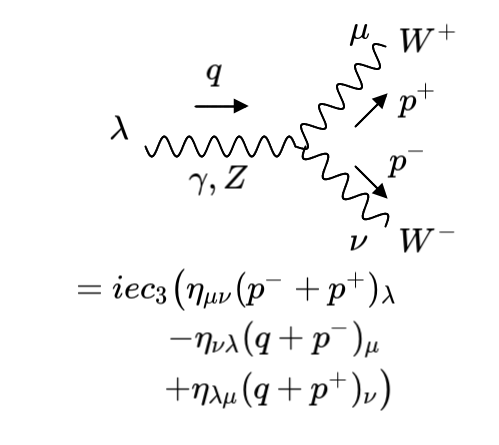
\includegraphics[width=0.5\textwidth]{figs/22a.png}}
  \hfill
  \subfloat[quartic vertex]{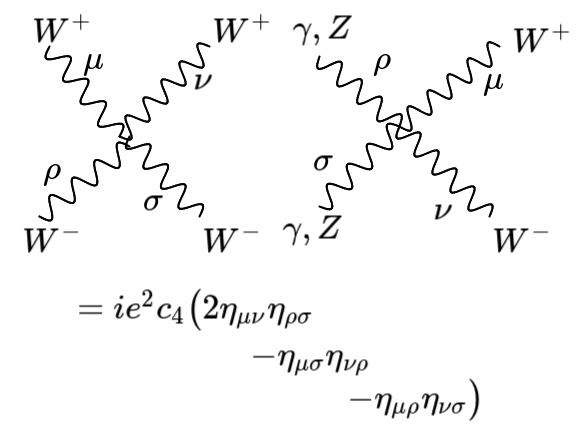
\includegraphics[width=0.5\textwidth]{figs/22b.png}}
\end{figure}
\newline
where 
\begin{equation}
c_3 =
\begin{cases}
1 \qquad \qquad \text{for } \gamma\\
\cot\theta_w \qquad \text{for } Z,
\end{cases}
\end{equation}
and

\begin{equation}
c_4 =
\begin{cases}
\csc^2\theta_w \qquad \text{for } WWWW\\
-1 \qquad \qquad \text{for } WW\gamma \gamma \\
-\cot\theta_w \qquad \text{for } WWZ \gamma \\
-\cot^2\theta_w \qquad \text{for } WWZZ.
\end{cases}
\end{equation}
Note that the photon couples to the electric charge of the $W^\pm$: there is no dependence on $\theta_w$. There are no couplings which only involve $\gamma$ and $Z^0$, as the $Z^0$ is neutral and $\gamma$ only couples to electrically charged particles. It is easy to show that $\mathcal{L}_{YM}$ is gauge invariant under U(1)$_Q$ if the $Z$ is ignored (Exercise). 
%
\subsection{The Z mass}
%
Clearly the $Z^0$ must be heavy, like $W^\pm$, otherwise the neutral current interactions would be long-range. We can introduce a mass term by hand, just as we did for the $W^\pm$, ensuring it is consistent with \textit{global} SU(2)$_L \otimes$U(1)$_Y$ symmetry. Remember that such a term will always break gauge invariance. The most general mass term is
\begin{equation}
\mathcal{L}_M  = m_W^2 W_\mu^\dagger W^\mu + \frac{1}{2} W_\mu^3 W_3^\mu + \frac{1}{2}m_B^2 B_\mu B^\mu.
\end{equation}
However, this can't be correct: the mass eigenstates are $Z_\mu$ and $A_\mu$, and the photon ($A_\mu$) is massless. We saw above that $W_\mu^3$ and $B_\mu$ mix. We can assume this mixing is in the mass matrix, which will mean it has no effect at high energy (where the masses are negligible). This is known as \textit{soft breaking}. In this case,
\begin{equation}
\mathcal{L}_{gauge}^{mass} \to \mathcal{L}_{gauge}^{mass} - m_X^2W_\mu^3 B^\mu,
\end{equation}
and we can write the mass matrix for $W_\mu^3$ and $B_\mu$ as:
\[ \left( \begin{array}{cc}
m_W^2 & -m_X^2  \\
-m_X^2 & m_B^2  \end{array} \right).  \]
We know because the photon is massless that this must have a zero eigenvalue. This fixes $m_X^2 = m_W m_B$. Moreover, we know that the corresponding zero eigenvector is
$A_\mu = \sin\theta_w W_\mu^3 + \cos\theta_w B_\mu$, so 
\[ \left( \begin{array}{cc}
m_W^2 & -m_Wm_B  \\
-m_Wm_B & m_B^2  \end{array} \right)
\left( \begin{array}{cc}
\sin\theta_w \\
\cos\theta_w \end{array} \right) = 0 \\
\implies m_B\cos\theta_w = m_W\sin\theta_w. \]
The other eigenvalue is 
\begin{equation}
\begin{split}
m_Z^2 &= m_W^2 + m_B^2 \\
&= m_W^2(1+ \tan^2\theta_w) \\
&= \frac{m_W^2}{\cos\theta_w} > m_W^2.
\end{split}
\end{equation}
Note that the fermion mass terms $\mathcal{L}_m = m(\bar{\psi}_L\psi_R + \bar{\psi}_R \psi_L)$ also break SU(2)$_L \otimes$U(1)$_Y$, and mix the SU(2) doublets (left-handed fermions) with the U(1) singlets (right-handed fermions). 
%
\subsubsection{Summary}
%
\begin{itemize}
\item SU(2)$_L \otimes$U(1)$_Y$ symmetry remains at high energy,
\item $g = e/\sin\theta_w$: QED and electroweak are unified,
\item we predict a new \textit{neutral current} weak interaction with mass $m_Z = m_W/\cos\theta_w$,
\item mass terms for both vector bosons and fermions break the SU(2)$_L \otimes$U(1)$_Y$ symmetry by mixing.
\end{itemize}
%
\subsection{Neutral Currents}
%
Neutral currents are \textit{chiral}: they involve both left-handed and right-handed components but not equally, and they can involve neutrinos. However, they do \textit{not} change flavour, e.g. they don't change electrons into neutrinos. We say that there are no "flavour changing neutral currents" (FCNCs). 

The $Z_0$ is heavy (in fact it is heavier than the $W^\pm$), and has the propagator
\begin{equation}
\Delta_Z^{\mu \nu} = \frac{i(-\eta^{\mu \nu} + k^\mu k^\nu/m_Z^2)}{k^2 - m_Z^2 + i \epsilon},
\end{equation}
and polarisation vectors $\epsilon_\mu^r(k)$, $r=1,2,3$ as for the $W$. At low energies $k^2 \ll m_Z^2$ and you end up with a new effective four-fermion interaction:
\newline
%\begin{wrapfigure}{l}{\linewidth}
  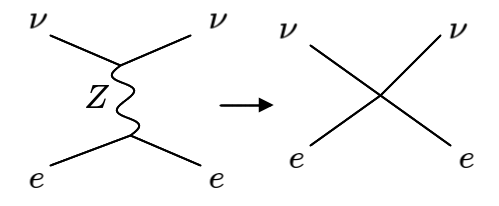
\includegraphics[width=0.6\linewidth]{figs/24a.png}
%\end{wrapfigure}
\newline
with an effective Lagrangian
\begin{equation}
\mathcal{L}_{4F} \to \frac{-g^2}{8m_W^2}(J_\mu^\dagger J^\mu + \rho J_\mu^{NC}J^\mu_{NC}),
\end{equation}
where $\rho = m_W^2/\cos^2\theta_w m_Z^2 =1$ is the Veltman parameter. Neutral current interactions are very difficult to see at low energy because of the  presence of the neutral electromagnetic current $\gamma$. Neutral current interactions were first observed at Garganelle (CERN) in 1973, in neutrino scattering off a nucleus: $\nu_\mu N \to \nu_\mu N$. These experiments are very difficult. The neutrino beam comes from pion decays. Early experiments found just 3 events in 2 years!
%
\subsubsection{Example: $\nu_\mu e^- \to \nu_\mu e^-$}
%
Let's first consider the process at low energy, as an effective theory.
\newline
%\begin{wrapfigure}{l}{\linewidth}
  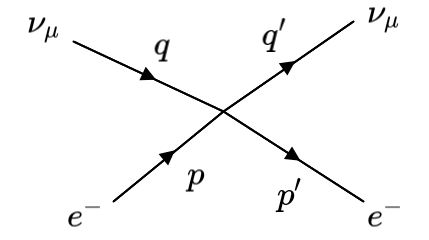
\includegraphics[width=0.4\linewidth]{figs/24b.png}
%\end{wrapfigure}
\newline
\begin{equation}
\mathcal{M} = \frac{-iG_F}{\sqrt{2}} \rho \bar{u}(p^\prime) \gamma_\mu(c_V - c_A \gamma^5) u(p) \bar{u}(q^\prime) \gamma^\mu (1-\gamma^5) u(q),
\end{equation}
so averaging over initial spins and summing over final spins gives
\begin{equation}
\begin{split}
\frac{1}{2}\sum_{spins}|\mathcal{M}|^2 &= \frac{G_F^2\rho^2}{4}\ tr \bigg(\slashed{p}^\prime \gamma_\mu(c_V-c_A\gamma^5)\slashed{p}\gamma_\nu(c_V-c_A \gamma^5)\bigg)\ tr \bigg(\slashed{q}^\prime \gamma^\mu(1-\gamma^5)\slashed{q}\gamma^\nu(1-\gamma^5)\bigg) \\
&= 8G_F^2 \rho^2 \bigg( (c_V^2+c_A^2)(p_\mu p^\prime_\nu + p^\prime_\mu p_\nu - \eta_{\mu \nu} p\cdot p^\prime) - 2ic_Vc_A \epsilon_{\mu \nu \alpha \beta}p^\alpha p^{\prime \beta}\bigg) \\
&\times \bigg(q^\mu q^{\prime \nu} + q^{\prime \mu} q^\nu -\eta^{\mu \nu} q \cdot q^\prime - i\epsilon^{\mu \nu \rho \sigma}q_\sigma q^\prime_\rho \bigg) \\
&= 16G_F^2 \rho^2 \bigg( (c_V^2+c_A^2)(p \cdot q p^\prime \cdot q^\prime + p\cdot q^\prime p^\prime \cdot q) + 2c_Vc_A(p \cdot q p^\prime \cdot q^\prime - p\cdot q^\prime p^\prime \cdot q) \bigg) \\
&= 16G_F^2 \rho^2 \bigg((c_V+c_A)^2 p \cdot q p^\prime \cdot q^\prime + (c_V-c_A)^2 p \cdot q^\prime p^\prime \cdot q \bigg) \\
&= 4 G_F^2\rho^2(c_L^2s^2 + c_R^2u^2)
\end{split}
\end{equation}
where we have used $c_L = c_V + c_A$ and $c_R = c_V-c_A$, and the Mandelstam variables $s=2 p \cdot q = 4E^2$ and $u=-2p \cdot q^\prime = -2E^2(1+ \cos\theta)$. We can now calculate the total cross section by integrating first over $\phi$ and then over $\theta$:
\begin{equation}
\begin{split}
\frac{d\sigma}{d\cos\theta} &= \frac{G_F^2 \rho^2}{2 \pi} E^2 \big(c_L^2 + c_R^2\frac{1}{2}(1 + \cos^2\theta)\big) \\
\implies \sigma(\nu_\mu e) &= \frac{G_F^2 \rho^2 E^2}{\pi} \big(c_L^2 + \frac{1}{3}c_R^2\big) \\
&= \frac{4G_F^2 \rho^2E^2}{3 \pi}\big(c_V^2 + c_A^2 + c_V c_A\big).
\end{split}
\end{equation}
You can infer $\sigma(\bar{\nu}_\mu e)$ from crossing symmetry $q \leftrightarrow q^\prime$, or $c_A \leftrightarrow -c_A$, $c_L \leftrightarrow c_R$. So the ratio of these two cross sections is
\begin{equation}
\frac{\sigma(\bar{\nu}_\mu e)}{\sigma(\nu_\mu e)} = \frac{c_V^2 + c_A^2 - c_Vc_A}{c_V^2 + c_A^2 + c_V c_A},
\end{equation}
where in this instance $c_V = 2 \sin^2\theta_w -1/2$ and $c_A = -1/2$. From measuring their rate experimentally, we can deduce that $\sin^2\theta_w \approx 0.23$. 

For the high-energy cross section we need to take account of the $Z^0$ propagator.
\begin{wrapfigure}{l}{0.3\linewidth}
  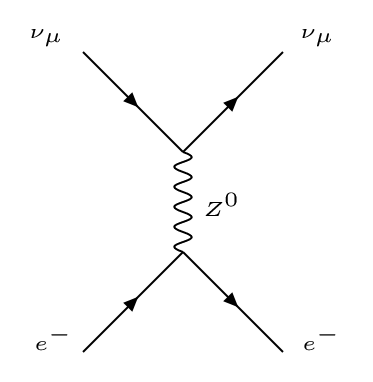
\includegraphics[width=\linewidth]{figs/25a.png}
\end{wrapfigure}
This corresponds to replacing 
\begin{equation}
-i\eta^{\mu\nu} \to i(-\eta^{\mu\nu} + k^\mu k^\nu/m_Z^2)/k^2-m_Z^2.
\end{equation} 
But remember that 
\begin{equation}
\bar{u}(q^\prime)\slashed{k}(1-\gamma^5)u(q) = \bar{u}(q^\prime)(\slashed{q}-\slashed{q}^\prime)(1-\gamma^5)u(q)=0,
\end{equation}
so in fact we can ignore the $k^\mu k^\nu/m_Z^2$ term, and only need to address the change in the denominator. 
\begin{equation}
k^2 = t = -2E^2(1-\cos\theta),
\end{equation}
so the total differential cross section becomes
\begin{equation}
\frac{d\sigma}{d\cos\theta} = \frac{e^4}{\pi\sin^2\theta_w}\frac{E^2}{(m_Z^2 + 2E^2(1-\cos\theta))^2}\big(c_L^2 + c_A^2 \frac{1}{2}(1+\cos\theta)^2\big).
\end{equation}
You can see that in this case unitarity is retained in the limit $E^2 \gg m_Z^2$.
%
\subsubsection{Example: $e^+ e^- \to \mu^+ \mu^-$}
%
\begin{figure}[!h]
  \centering
  \subfloat[QED]{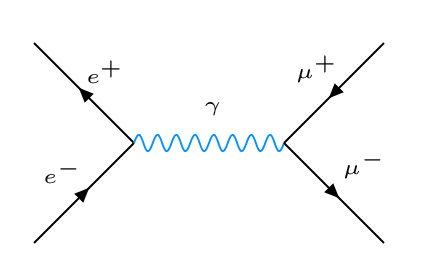
\includegraphics[width=0.5\textwidth]{figs/25b.png}}
  \hfill
  \subfloat[NC]{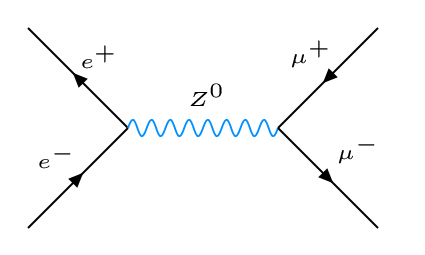
\includegraphics[width=0.5\textwidth]{figs/25c.png}}
\end{figure}
This is a standard process occurring at $e^+ e^-$ colliders, and is a very sensitive test of NC electroweak theory. See the examples sheet.
%
\subsubsection{Example: $\nu \bar{\nu} \to W^+W^-$ again}
%
We saw earlier that the diagram in the $t$-channel violates unitarity. We now have a new graph in the $s$-channel, representing the contribution from the $Z^0$.
\begin{figure}[!h]
  \centering
  \subfloat[$t$-channel]{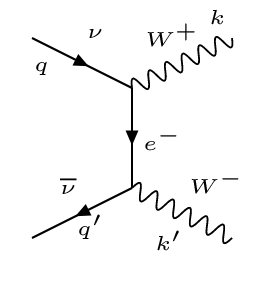
\includegraphics[width=0.3\textwidth]{figs/26a.png}}
  \hfill
  \subfloat[$s$-channel]{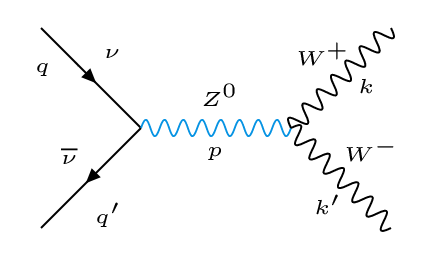
\includegraphics[width=0.5\textwidth]{figs/26b.png}}
\end{figure}
Does the addition of this diagram restore unitarity? We need to compute the total amplitude $\mathcal{M} = \mathcal{M}_t + \mathcal{M}_s$. We already worked out that
\begin{equation}
\mathcal{M}_t = \frac{+ig^2}{4m_W^2}\bar{v}(q^\prime)\slashed{k}(1-\gamma^5)u(q),
\end{equation}
and we can use the Feynman rules in the $s$-channel to write
\begin{equation}
\begin{split}
\mathcal{M}_s = \frac{+ig}{4\cos\theta_w}\bar{v}(q^\prime)\gamma_\mu(1-\gamma^5)u(q)i\frac{-\eta^{\mu \nu}+p^\mu p^\nu/m_Z^2}{p^2-m_Z^2}(ig\cos\theta_w) \\
\times \bigg(\eta_{\alpha \beta}(k^\prime - k)_\nu - \eta_{\beta \nu} (p + k^\prime)_\alpha + \eta_{\alpha \nu}(p+k)_\beta \bigg)\frac{k^\alpha}{m_W}\frac{k^{\prime \beta}}{m_W},
\end{split}
\end{equation}
where we have used the high energy limits to simplify the external $W$ lines, and that, for $\nu$, $c_V = c_A = 1/2$.

Let's look first at the $p^\mu p ^\nu$ term, using $p=q+q^\prime = k + k^\prime$ and matching up all the indices:
\begin{equation}
\begin{split}
&(k \cdot k^\prime) p \cdot(k^\prime - k) - (p \cdot k^\prime)(p+k^\prime)\cdot k + (p \cdot k)(p+k) \cdot k^\prime \\
=\ &(k \cdot k^\prime)p\cdot(k^\prime-k) + k\cdot k^\prime (p\cdot k - p \cdot k^\prime) \\
=\ &0.
\end{split}
\end{equation}
So we are just left with the $-\eta^{\mu \nu}$ term:
\begin{equation}
\begin{split}
&- \big( (k \cdot k^\prime)(k^\prime_\mu - k_\mu) - k_\mu^\prime (p+k^\prime)\cdot k + k_\mu (p+k)\cdot k^\prime \big) \\
=\ &p \cdot k k^\prime_\mu - p \cdot k^\prime k_\mu,
\end{split}
\end{equation}
but 
\begin{equation}
\bar{v}(q^\prime)\slashed{k}^\prime(1-\gamma^5)u(q) = -\bar{v}(g^\prime)\slashed{k}(1-\gamma^5)u(q),
\end{equation}
so altogether
\begin{equation}
\mathcal{M}_s = -\frac{ig}{4m_W^2}v(q^\prime)\slashed{k}(1-\gamma^5)u(q) \frac{p \cdot (k + k^\prime)}{p^2-m_Z^2},
\end{equation}
and
\begin{equation}
\begin{split}
\mathcal{M}_t + \mathcal{M}_s = \frac{ig^2}{4m_W^2}\bar{v}(q^\prime)\slashed{k}(1-\gamma^5)u(q)\bigg(1-\frac{p^2}{p^2-m_Z^2}\bigg).
\end{split}
\end{equation}
The bracketed term on the right can be re-expressed as $-m_Z^2/(p^2-m_Z^2) = -m_Z^2/(s-m_Z^2)$, so 
\begin{equation}
\mathcal{M}_t + \mathcal{M}_s = -{ig^2}{4\cos^2\theta_w}\frac{1}{s-m_Z^2}\bar{v}(q^\prime)\slashed{k}(-\gamma^5)u(q).
\end{equation}
Squaring as before, we arrive at
\begin{equation}
\frac{d\sigma}{d\Omega} = \frac{g^4}{64\pi^2\cos\theta_w}\frac{ut-m_W^4}{s(s-m_Z^2)^2},
\end{equation}
so for $E^2 \gg m_W^2$
\begin{equation}
\frac{d\sigma}{d\cos\theta} = \frac{1}{16E^2}\frac{g^4\sin^2\theta}{128\pi\cos^4\theta_w}.
\end{equation}
Thankfully, unitarity is restored! (N.B. Remember that we took the high energy limit in the $\epsilon_\mu$ terms for external $W$ bosons. The sub-leading terms give an additional factor of $\cos^22\theta_w$.) 

However, there are still processes which violate unitarity, such as $W^+W^- \to W^+W^-$. There is also no improvement in the issue of power-counting renormalisability. 
%
\subsection{Hadronic Neutral Current}
%
Remember the expression for hadronic charged current:
\begin{equation}
\frac{1}{2}J_\mu^h = \bar{u}_L \gamma_\mu d^\prime_L + ...,
\end{equation}
so we have left-handed doublets
\[ q_L = \left( \begin{array}{cc}
u   \\
d^\prime   \end{array} \right)_L, \qquad
  \\ \left( \begin{array}{cc}
 c \\
s^\prime   \end{array} \right)_L, \qquad  \\ 
\left( \begin{array}{cc}
 t \\
b^\prime   \end{array} \right)_L; \qquad\] 
and right-handed singlets $q_R = u_R, d_R, c_R, s_R, t_R, b_R$.  So
\begin{equation}
\underline{J}^h_\mu = \bar{q}_L \underline{T} \gamma_\mu q_L,
\end{equation}
i.e.
\begin{equation}
J_\mu^{3\ h} = \frac{1}{2}\bar{u}_L \gamma_\mu u_L - \frac{1}{2} \bar{d}_L^\prime \gamma_\mu d_L^\prime + ...,
\end{equation}
while the electromagnetic current is
\begin{equation}
j_\mu^h = \frac{2}{3} \bar{u} \gamma_\mu u - \frac{1}{3} \bar{d}^\prime \gamma_\mu d^\prime + ...,
\end{equation}
corresponding to 
\[ Q = \left( \begin{array}{cc}
2/3 & 0   \\
0 & -1/3   \end{array} \right). \qquad \]
Using this to evaluate the weak hypercharge,
\begin{equation}
Y = Q - T_3 =
\begin{cases}
+\frac{1}{6}\mathds{1} \qquad \qquad \text{for LH doublets} \\
+\frac{2}{3} \qquad \qquad \text{  for } u_R, c_R, t_R \\
-\frac{1}{3} \qquad \qquad \text{  for } d_R, s_R, b_R. 
\end{cases}
\end{equation}
The netural-current can then be expressed:
\begin{equation}
\begin{split}
J_\mu^{NC\ h} &= 2 (J_\mu^{3\ h} - \sin^2\theta_w j_\mu^h) \\
&= 2 \bar{q} \gamma_\mu \bigg(\frac{1}{2} T_3 (1-\gamma^5) - Q \sin^2\theta_w \bigg) q \\
&= \bar{u} \gamma_\mu \bigg( -\frac{4}{3}\sin^2\theta_w + \frac{1}{2}(1-\gamma^5)\bigg) u + \bar{d}^\prime \gamma_\mu \bigg(\frac{2}{3} \sin^2\theta_w - \frac{1}{2}(1 - \gamma^5) \bigg) d^\prime + ...
\end{split}
\end{equation}
This corresponds to the Feynman rule
\newline
  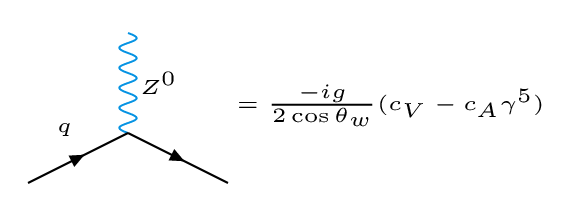
\includegraphics[width=0.7\linewidth]{figs/27a.png}
\newline
where for up-type quarks,
\begin{equation}
c_V = -\frac{4}{3}\sin^2\theta_w + \frac{1}{2}, \qquad c_A = \frac{1}{2};
\end{equation}
and for down-type quarks,
\begin{equation}
c_V = \frac{2}{3}\sin^2\theta_w - \frac{1}{2}, \qquad c_A = -\frac{1}{2}.
\end{equation}
%
\subsection{The GIM Mechanism - Glashow, Illiopoulos, Maiani (1970)}
%
For now let's consider only the light quarks $u$, $d$ and $s$. The down-type quarks are in general mixtures of the down-type components of the left-handed doublets. We can express this "Cabbibo mixing" using the Cabbibo angle $\theta_c$:
\begin{equation}
d^\prime = \cos\theta_c + \sin\theta_c.
\end{equation}
Then the neutral-current term $\bar{d}^\prime \gamma_\mu (c_V - c_A \gamma^5) d^\prime \equiv \bar{d}^\prime \Gamma d^\prime$, contains $\Delta Q = 0, \Delta S = 1$ pieces:
\begin{equation}
\sin\theta_c \cos\theta_c (\bar{d} \Gamma s + \bar{s} \Gamma d) .
\end{equation}
These are "flavour changing neutral currents" (FCNCs). The existence of these in the theory is embarrassing, because in actual fact $s \to d \nu \bar{\nu}$ never happens. There are experimental constraints set by Kaon decay rates:
\begin{equation}
\frac{\Gamma(K^+ \to \pi^+ \nu \bar{\nu})}{\Gamma(K^+ \to \text{all})} < 10^{-7}, \qquad \frac{\Gamma(K^0 \to \pi^+ \mu^+ \mu^-)}{\Gamma(K^0 \to \text{all})} < 10^{-8}.
\end{equation}
The solution is via the introduction of the charm quark, $c$. Then $\icol{c\\s^\prime}_L$ is an SU(2)$_L$ doublet, and if $s^\prime = -\sin\theta_L d + \cos \theta_c s$, the FCNCs cancel:
\begin{equation}
\bar{d}^\prime \Gamma d^\prime + \bar{s}^\prime \Gamma s^\prime =\bar{d} \Gamma d + \bar{s} \Gamma s.
\end{equation}
So with two generations (for three generations see later in the course), 
\[\left( \begin{array}{cc}
d^\prime \\
s^\prime 
\end{array} \right) =
 \left( \begin{array}{cc}
\cos\theta_c & \sin\theta_c \\
-\sin\theta_c & \cos\theta_c  \end{array} \right) 
\left( \begin{array}{cc}
d \\
s
\end{array} \right). \]
This predicted the existence of the charm quark, which was discovered in the form of the $J/\psi$ particle, a bound $c\bar{c}$ state of mass 3 GeV, in 1974 at SLAC/BNL.
%
\subsection{The Discovery of $W$ and $Z$}
%
The $W$ and $Z$ were discovered at SPS and CERN in 1983. They are easiest to produce in hadronic collisions.
\begin{figure}[!h]
  \centering
  \subfloat[$W$]{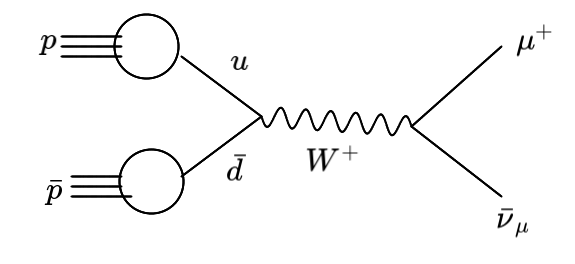
\includegraphics[width=0.4\textwidth]{figs/27b.png}}
  \hfill
  \subfloat[$Z$]{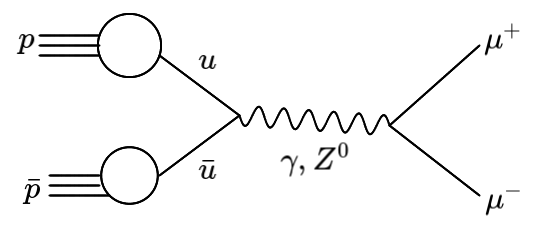
\includegraphics[width=0.4\textwidth]{figs/27c.png}}
\end{figure}
The partonic cross-sections are easy to calculate. The properties of the $Z^0$ in particular were explored with great precision at LEP (an $e^+ e^-$ collider operating from 1989-2001). The $Z^0$ has a very clean final state signature, unlike the $W$ where the neutrino is not visible to the detectors. 
